% $Header: /projects/VU-SAGA/Papers/saga_engine_2006/details.tex,v 1.17 2006/10/11 02:55:39 gallen Exp $

The following section will describe certain implementation details
of the SAGA C++ reference implementation. As will be described, the 
implementation gains its flexibility mainly from the combined
application of C++'s compile time and runtime polymorphism features,
i.e.\ template's and virtual functions respective.

\subsection{General Considerations}

  To achieve  maximum portability, platform independence and code
  reuse, the SAGA C++ reference implementation relies strictly on the
  Standard C++ language features, and uses the C++ Standard and Boost
  libraries where possible. 
  
\subsubsection{The SAGA task model}
\label{ssec:tasks}

  A central concept of the SAGA API design is the SAGA task
  model~\cite{saga-paper}, prescribing
  the form of
  synchronous and asynchronous method calls.  Essentially, each method
  call comes in three variants: as a \I{synchronous call} (executed 
  immediately), as a \I{asynchronous call}, and as a \I{task call}.  
  The latter versions of the calls return a \T{saga::task} class instance.  A
  \T{saga::task} thus represents an asynchronously running operation,
  and has an associated state (\T{New, Run\-ning, Finished, Failed}).  Task versions
  of the method calls return a \T{New} task, asynchronous versions
  return a \T{Run\-ning} task. %, i.e. the \T{run()} method was called on
  %that task.  
  For symmetry reason, we added a fourth, synchronous version of method
  calls, returning a \T{Finished} task.
  % i.e. \T{run()} and \T{wait()} have been called.
  The realization of the |saga::impl::task| class bases on a
  implementation of the \I{futures} paradigm, a concurrency abstraction 
  first proposed for MultiLisp~\cite{futures}.  
  The C++ rendering of the SAGA task model is shown in
  figure~\ref{src:tasks}.

\begin{figure}[!ht]
 \begin{center}
  \begin{mycode}[label=SAGA task model]
    string dest = "any://host.net//data/dest.dat";
    file   file  ("any://host.net//data/src.dat");

    // normal sync version of the copy method
    file.copy (dest);

    // the three task versions of the same method
    task t1 = file.copy <task::Sync>  (dest);
    task t2 = file.copy <task::ASync> (dest);
    task t3 = file.copy <task::Task>  (dest);

    // task states of the returned saga::task
    // t1 is in 'Finished' or 'Failed' state
    // t2 is in 'Running'              state
    // t3 is in 'New'                  state

    t3.run  ();
    t2.wait ();
    t3.wait ();
    // all tasks are 'Finished' or 'Failed' now
  \end{mycode}
  \up
  \up
  \caption{\label{src:tasks}
    The SAGA task model rendered in C++}
 \end{center}
\end{figure}

While we tried to absolutely minimize the use of template's in the 
API layer, it was decided to implement the different flavors of the API 
functions using function templates (see figure~\ref{src:tasks}). 
This makes the whole SAGA C++ implementation \I{generic} with respect to 
the synchronicity model, being another reason for providing 
two types of the synchronous function flavors: a direct and a task 
based one.

\subsubsection{The Object Instance Structure}
\label{ssec:pimpl}

As already mentioned, the SAGA API objects are implemented using the PIMPL idiom.
Their only essential member is a \T{boost::smart\_ptr<>} to the 
base class of the implementation object instance\footnote{\small We refer to the 
implementation side of the PIMPL layer as \I{impl classes} in this document}, 
keeping it alive. This makes them very 
lightweight and copyable without major overhead, and therefore storable in any 
type of container.

\begin{figure}[!ht]
 \begin{center}
  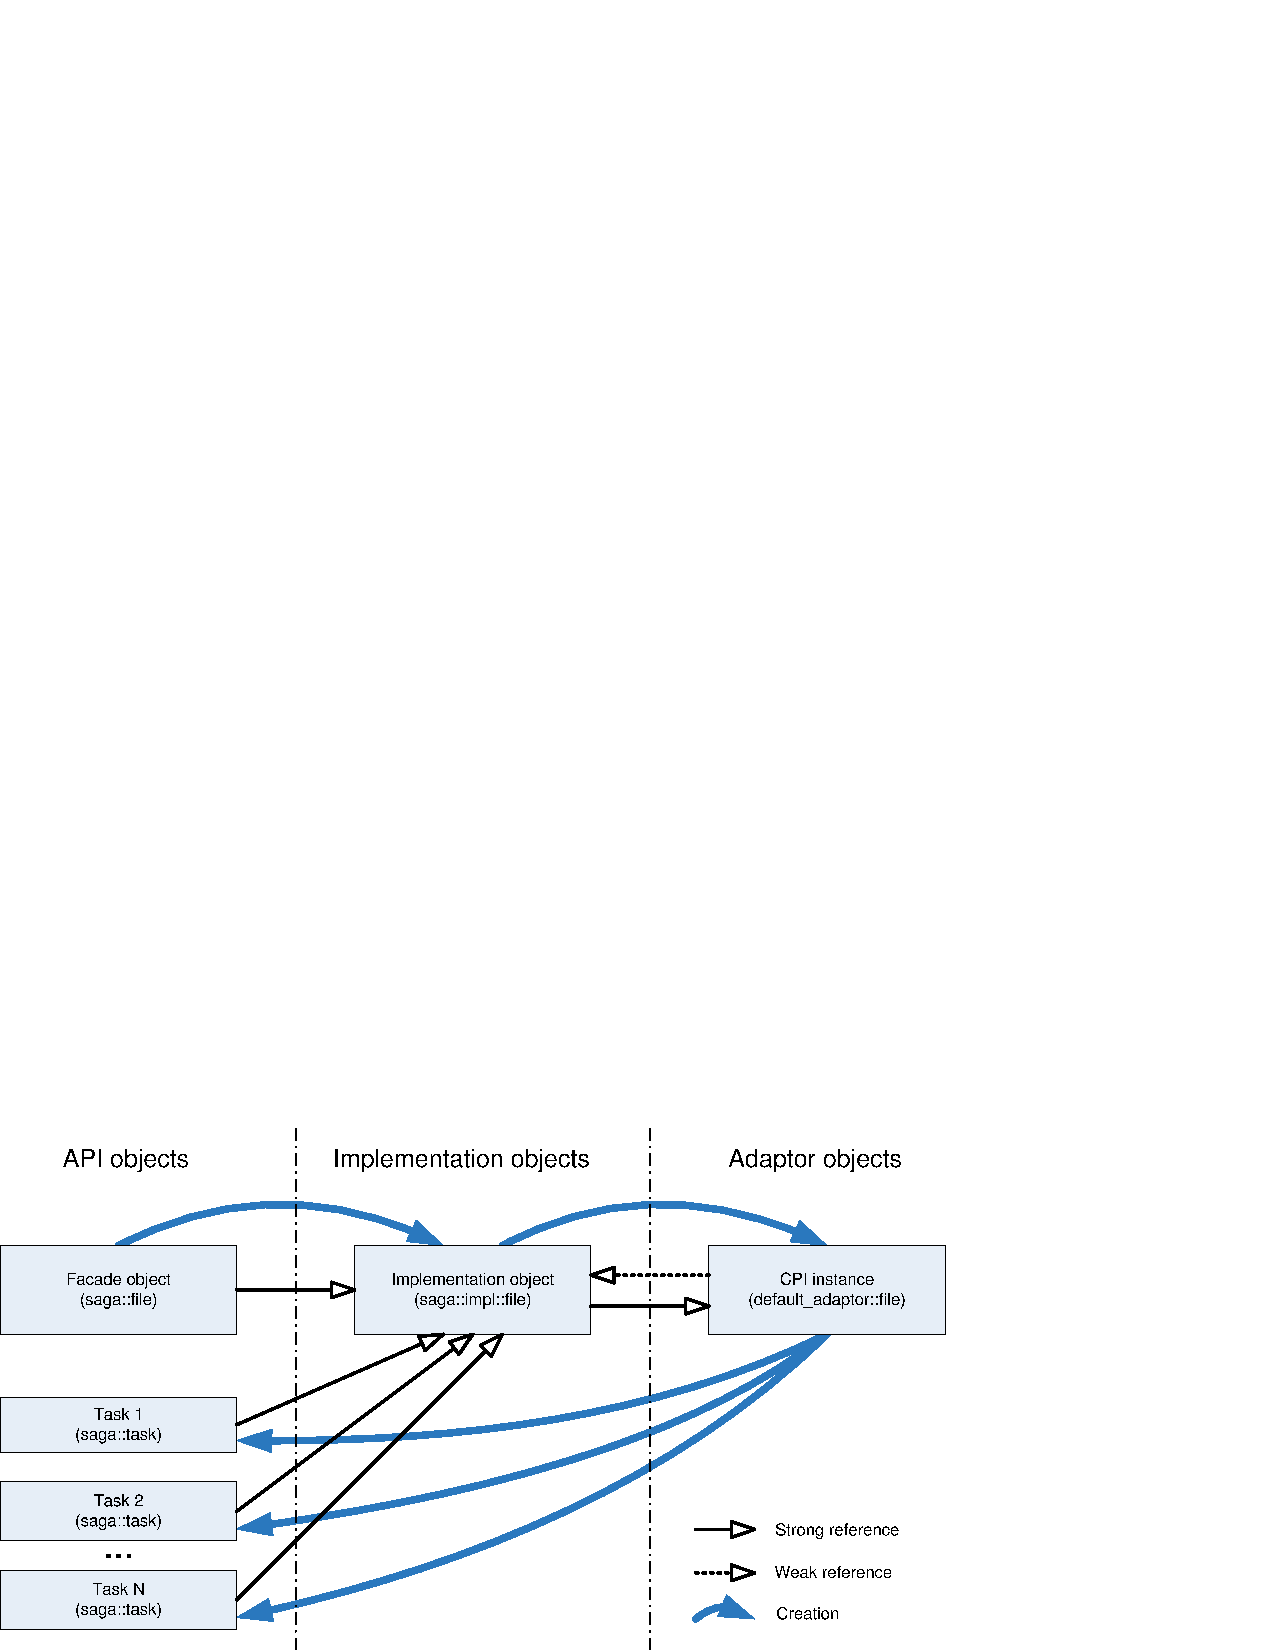
\includegraphics[width=0.47\textwidth]{images/object_structure}
  \up
  \caption{\label{fig:object_structure}
    Object instance structure: Copying a API object instance means sharing 
    state, returned tasks keep implementation alive.}
 \end{center}
\end{figure}

As shown in figure~\ref{fig:object_structure}, any API object instance creates
the corresponding impl instance holding all the instance data
of the SAGA object instance 
Copying of an API instance therefore shares this state between the copied 
instances.
This behavior is consistent with anticipated handle based SAGA language bindings 
(e.g. in C or FORTRAN), where copying the handle representing a SAGA 
object instance naturally means sharing the internal instance data as 
well\footnote{\small A polymorphic \T{saga::object::clone()} method is, however, part 
of the SAGA API, and allows for explicit deep copies of API objects, 
forcing the instance data to be copied as well.}.  

Due to the shared
referencing after copies, the impl instances can be kept alive by objects
which depend on their state -- for example, a task keeps the objects
alive for which they represent a asynchronous method call (see
figure~\ref{fig:object_structure}).

The call sequence for creating a SAGA API object instance is shown in
figure~\ref{fig:object_creation}.  Whenever needed, the implementation
creates a CPI object instance implemented in one of the adaptors.
The process of adaptor selection and CPI instantiation is injected into the 
API packages by the macros mentioned before (see section~\ref{ssec:apipackages}).

\begin{figure}[!ht]
 \begin{center}
  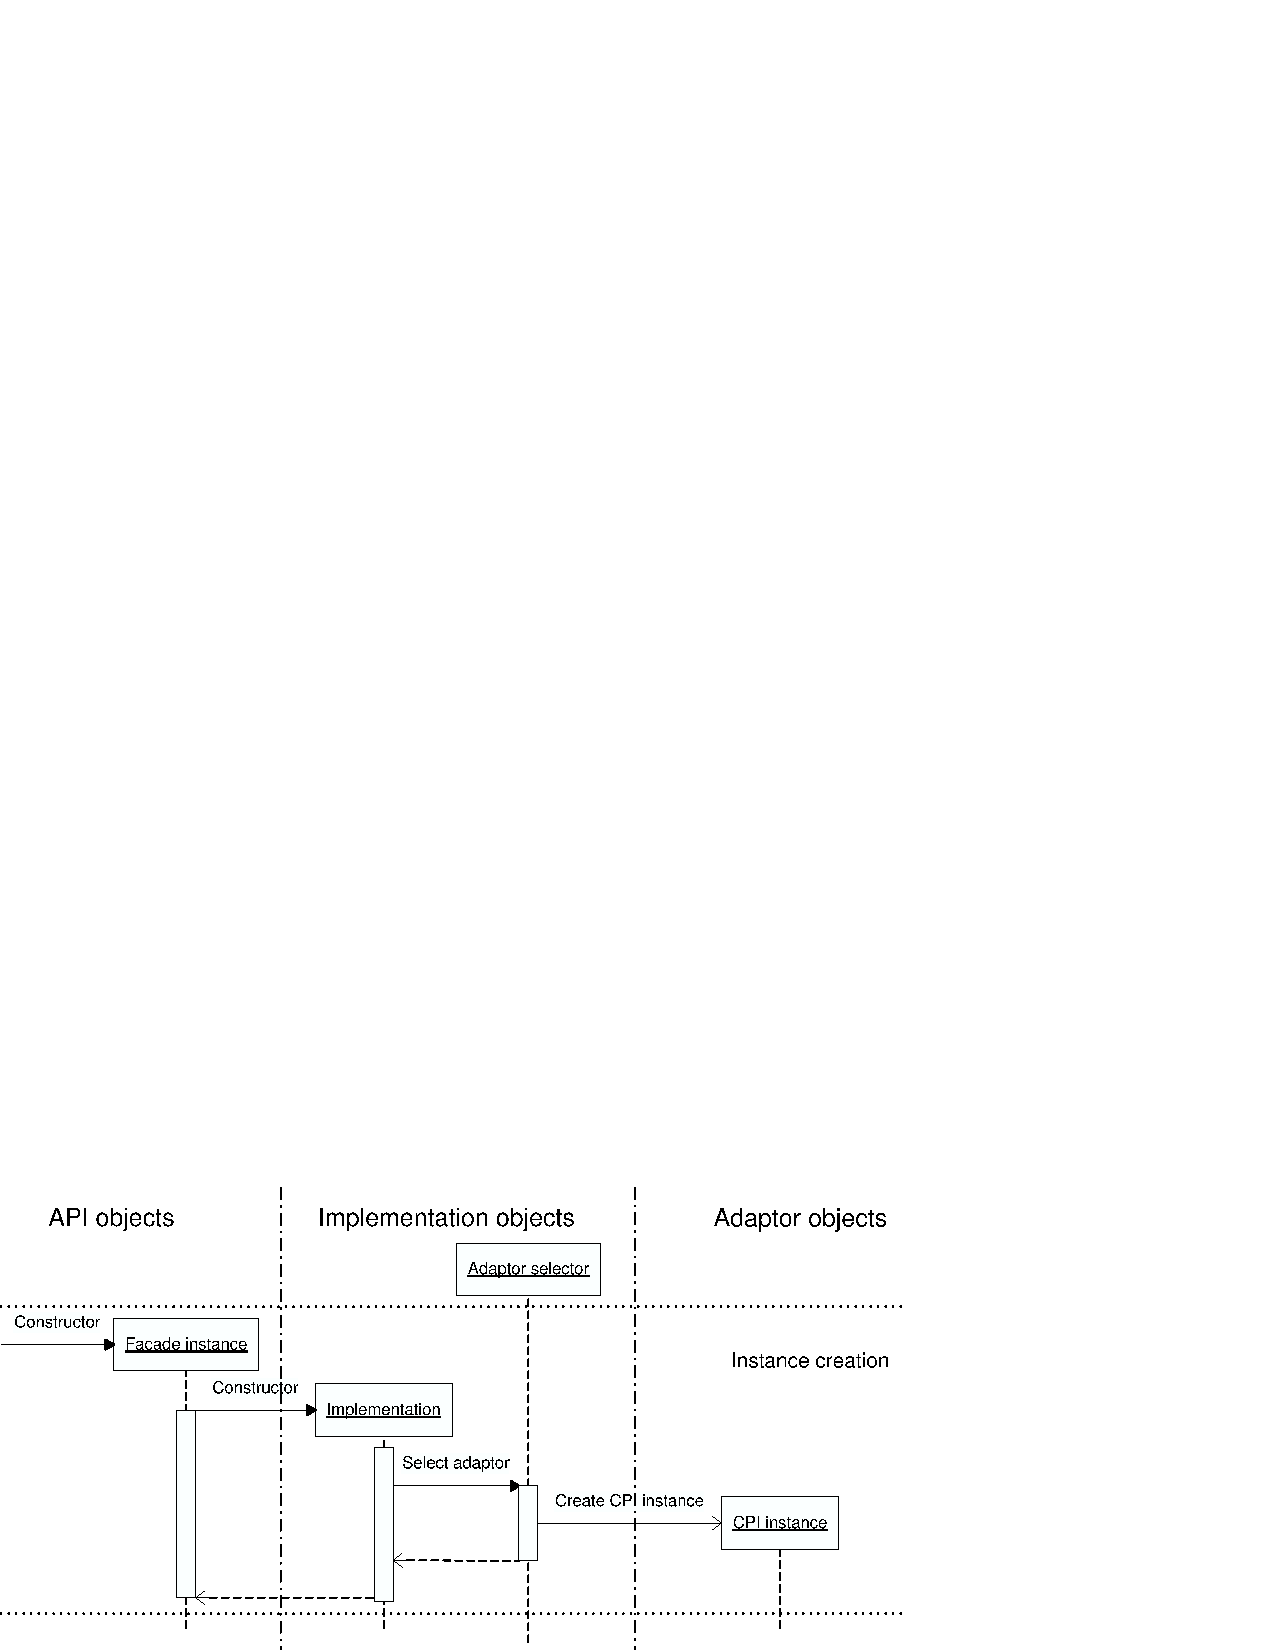
\includegraphics[width=0.47\textwidth]{images/object_lifetime_creation}
  \up
  \caption{\label{fig:object_creation}
    Object creation: Sequence diagram depicting the creation of all
    components as showed in figure~\ref{fig:object_structure}. Note, how
    the call is intercepted by a SAGA engine module component to select 
    a appropriate adaptor.}
 \end{center}
\end{figure}

\up
\up
\subsection{Inheritance and PIMPL}

An interesting problem in the strict application of the PIMPL
mechanism lies in the API object hierarchy:  the \T{saga::file} class
for example inherits the \T{saga::ns\_entry} class, which inherits the
\T{saga::object} class.  Additionally, the SAGA specification requires
all these classes to implement additional interfaces.  Now, the PIMPL
paradigm requires all class instances to own exactly \I{one} impl
pointer\footnote{\small{In fact the impl pointer stored in any \T{saga::object}
instance is a \T{boost::smart\_ptr<saga::impl::object>}, i.e. a reference
to the very base class of the implementation object hierarchy.}}, and are 
built using single inheritance only, otherwise we would face object slicing 
problems when copying around the base classes only. The solution is (1) to
add the required interfaces to the most derived classes by duplication
the interface functions, and (2) to up-cast the impl reference stored in the
base class whenever needed.

\begin{figure}[!ht]
 \begin{center}
  \begin{mycode}[label=Constructors in the saga::file hierarchy]
  // saga::file constructor
  file::file ([args])
  :  ns_entry (new saga::impl::file ([args]))  {}
  
  // saga::ns_entry constructor
  ns_entry::ns_entry (saga::impl::ns_entry* impl)
  :  saga::object (impl) {}
  
  // saga::object constructor
  //  'impl_' is a boost::smart_ptr<saga::impl::object>
  object::object (saga::impl::object* impl)
  :  impl_ (impl) {}
  \end{mycode}
  \up
  \up
  \caption{\label{src:implcon}
    Realizing inheritance in PIMPL classes (simplified).  Only the
    \T{saga::object} base class owns an impl pointer.}
 \end{center}
\end{figure}

API classes access the impl pointer through \T{get\_impl()}, which, in
derived classes, implies a static up-cast for the base class' impl
pointer.  

The implementation objects resemble the API object hierarchy.  These
are also derived from a common base class and contain, somewhere in
their own hierarchy, similar objects to the API objects.  The
\T{saga::impl::file} class\footnote{\small{The \T{saga::impl::file}
class for example is the implementation equivalent to the
\T{saga::file} class, as we kept all API classes in \T{namespace~saga}
and all corresponding implementation classes in
\T{namespace~saga::impl}.}} inherits the \T{saga::impl::ns\_entry}
class, which inherits the implementation specific
\T{saga::impl::proxy} class, which is derived from the common
\T{saga::impl::object} class.  Thus, the class hierarchy on the
implementation side of the PIMPL paradigm reflects the API side of the
class hierarchy, ensuring the correct casting behavior in the
\T{get\_impl()} methods.


\subsection{State Management}

Section~\ref{ssec:pimpl} discussed object state, in relation to
state sharing of objects after shallow copies.  Here we describe the object
state management of the SAGA implementation in more detail, since state
management is a central element on several layers.
On a different layer, the adaptors represent
operations on the object instances, and need to maintain state as well.
At the adaptor level this is complicated by the fact that the object state can (and in
general will) be changed by several adaptors (remember: adaptors are selected
at runtime, and may change for each API function invocation).  For state 
management, we hence distinguish between three types of state information.

\begin{shortlist}
	\item \I{Instance data} represent the state of API objects (e.g. file name, 
			file pointer etc.). These are predefined and not amendable by the adaptor
			as they represent common data either passed from the constructor,
			or needed for consistent state management on the API level.
	\item \I{Adaptor data} represent the state of CPI objects (e.g. open connections)
      and are shared between all instances of all CPI object types
			implemented by 
			a single adaptor and corresponding to a single adaptor instance. 
	\item \I{Adaptor-instance data} represent the state shared between all CPI 
			instances created for a single API object and implemented by the same 
			adaptor (e.g. remote handles). 
\end{shortlist}

The lifetime of any type of the state information is maintained by the SAGA engine 
module, which significantly simplifies the writing of adaptors.

All three types of state information are carefully protected from race 
conditions potentially caused by the multithreaded nature of the implementation.
We provide helper classes simplifying the 
correct locking of the instance data. 
This uniform state management enables 
object state persistency in the future, with minimal impact on the 
code base.

\subsection{Generic Call Routing}
\label{ssec:routing}

The essential idea of the implemented generic API call
routing mechanism is to represent the calls as abstract objects, and
to redirect their execution depending on several attributes 
and the adaptor suitability.  For example,
an asynchronous method call for a |saga::file| instance is preferably
directed to a asynchronous file adaptor, or, if such is not available,
to a synchronous file adaptor, wrapping it in a thread,
or, returns an error otherwise (|NotImplemented|).

This routing mechanism allows for (1) trivial (synchronous) adaptor 
implementations, (2) late binding (differents adaptor can be selected
for each call, even on the same API object instance), (3) variable adaptor 
selection strategies (based on adaptor meta data, user preferences, 
and heuristics), and (4) latency hiding (bulk optimization~\cite{CS_Hirmer_06a}, 
or automatic load distribution over multiple adaptors). 
Figure~\ref{fig:object_functioncall} is depicting the injection of the
call routing mechanism by the SAGA engine.

\begin{figure}[!ht]
 \begin{center}
  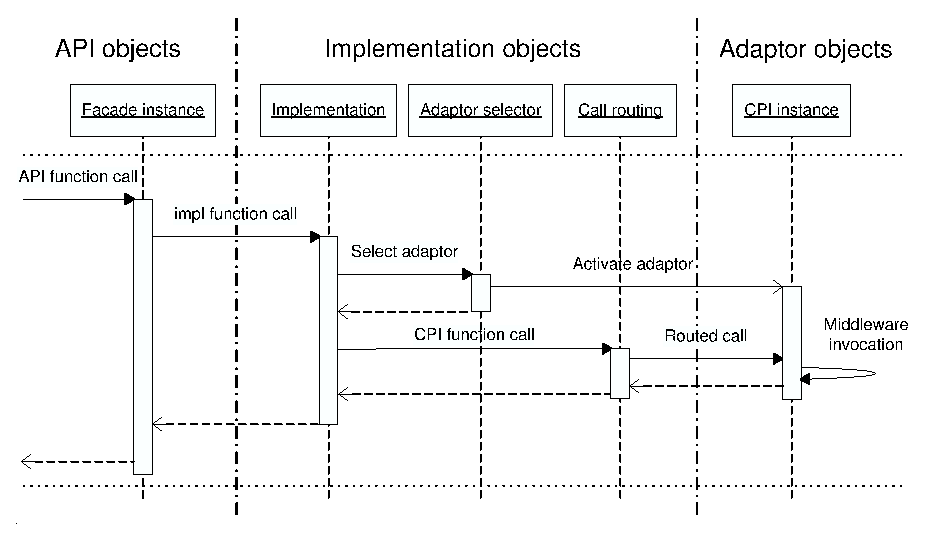
\includegraphics[width=0.47\textwidth]{images/object_lifetime_functioncall}
  \up
  \caption{\label{fig:object_functioncall}
    API function call: Diagram illustrating the execution sequence through 
    the different object instances during a call to any adaptor supplied 
    function.}
 \end{center}
\end{figure}

\up
All SAGA API methods come in synchronous and asynchronous flavors
(see section~\ref{ssec:tasks}).
To avoid, that adaptors need to implement
both flavors, we provide fallback implementations in the
SAGA engine.
The synchronous behavior is modelled by 
executing the the asynchronous implementation and waiting
for it to finish.  The asynchronous wraps the synchronous
implementation into a thread representing the asynchronous 
remote operation.

Even if this approach has a couple of drawbacks (it is not really asynchronous,
the middleware call still blocks, causing lock problems if implemented badly, and
tasks are not able to survive the application life time), the mechanism 
simplifies adaptor implementations
greatly, as most of the existing grid middleware is \I{not}
fully asynchronous anyway.

\subsection{Adaptor Selection}

The selection of suitable adaptors at runtime  is a central
component in the implementation (see
figure~\ref{fig:object_functioncall}).  It is, a very simple
mechanism: on loading, the adaptor components register their
\I{capabilities} in the adaptor registry.  If a method is to be
executed, the adaptor selector searches that registry for all 
suitable adaptors, orders them, and tries them one-by-one,
until the method invocation succeeds. The adaptor selection is 
routed through SAGA engine, generically implementing this for 
any API function.

To overcome the limitations of this approach (several CPI instances 
have to be created, remote operations add  additional latencies), our 
library allows adaptors to specify additional, key/value
based meta data, and also allows to exchange the adaptor selection
component.

\subsection{Utilization of Macros}
\label{ssec:macros}

Our SAGA implementation makes extensive use of C++ preprocessor
macros.  This might be perceived as a design flaw, at least by
some readers, and we were very hesitant to utilize macros
extensively.  However, the benefits for the end user
and other programmers(!) seem currently to outweigh the problems, 
such as limited debugging abilities.
mentioned in section~\ref{ssec:apipackages}, We are using Boost.Wave~\cite{boost_website}
features to pre-generate partially macro expanded sources to overcome 
the disadvantages of plain macros, hence simplifying debugging and 
improving readability.
